\documentclass{beamer}
\usepackage[utf8]{inputenc}
\usepackage{listings}
\usepackage{amsmath}
\usepackage{graphicx}
\usepackage{tikz}
\usepackage{pgfplots}

\DeclareFontShape{OT1}{cmss}{b}{n}{<->ssub * cmss/bx/n}{} 
%\usepackage{bm}
%\usepackage{esvect}
%\usepackage{mathrsfs}
%\usepackage{mathtools}
%\usepackage{subcaption}
\usepackage{url}
\usepackage{tikz}
\usepackage{tkz-euclide} % loads  TikZ and tkz-base
%\usetkzobj{all}
\usetikzlibrary{calc,math}
\usepackage{float}
\newcommand\norm[1]{\left\lVert#1\right\rVert}
%\renewcommand{\vec}[1]{\mathbf{#1}}


\usepgfplotslibrary{external}
\tikzexternalize
\pgfplotsset{compat = 1.9}
\usetheme{Boadilla}
\lstset{
%language=C,
frame=single, 
breaklines=true,
columns=fullflexible
}

\providecommand{\pr}[1]{\ensuremath{\Pr\left(#1\right)}}
\providecommand{\qfunc}[1]{\ensuremath{Q\left(#1\right)}}
\providecommand{\sbrak}[1]{\ensuremath{{}\left[#1\right]}}
\providecommand{\lsbrak}[1]{\ensuremath{{}\left[#1\right.}}
\providecommand{\rsbrak}[1]{\ensuremath{{}\left.#1\right]}}
\providecommand{\brak}[1]{\ensuremath{\left(#1\right)}}
\providecommand{\lbrak}[1]{\ensuremath{\left(#1\right.}}
\providecommand{\rbrak}[1]{\ensuremath{\left.#1\right)}}
\providecommand{\cbrak}[1]{\ensuremath{\left\{#1\right\}}}
\providecommand{\lcbrak}[1]{\ensuremath{\left\{#1\right.}}
\providecommand{\rcbrak}[1]{\ensuremath{\left.#1\right\}}}

\let\vec\mathbf

\newcommand{\myvec}[1]{\ensuremath{\begin{pmatrix}#1\end{pmatrix}}}
\newcommand{\mydet}[1]{\ensuremath{\begin{vmatrix}#1\end{vmatrix}}}

\title{Modeling Tweet Arrival Times using Log-Gaussian Cox Processes}
\author{Debolena Basak - AI20RESCH11003}
\date{}

\begin{document}
\begin{frame}
\titlepage
\end{frame}

\begin{frame}
\frametitle{Abstract}
\begin{block}{}
\begin{enumerate}
    \item This paper focuses on predicting when the next tweet event will occur.
    \item It is modeled and predicted using \textbf{Log Gaussian Cox Process(LGCP)}.
    \item LGCP - an inhomogeneous Poisson Process which captures the varying rate at which the tweets arrive over time.
    \item Incorporating textual features further improves predictions.
\end{enumerate}
\end{block}
\end{frame}

\begin{frame}{Motivation}
\begin{enumerate}
    \item Modeling the temporal dynamics of tweets provides useful information about the evolution of events.
    \item Inter-arrival time prediction is a type of such modeling and has application in many settings like real-time disaster monitoring, journalism(tracking rumours) and advertising on social media.
    \item Modeling the inter-arrival time of tweets is a challenging task due to complex temporal patterns exhibited.
    \item Tweets associated with an event stream arrive at different rates at different points in time.
    \item So the authors address the inter-arrival time prediction problem with \textbf{log-Gaussian Cox process(LGCP)}.
\end{enumerate}
\end{frame}

\begin{frame}{Introduction}
\begin{enumerate}
    \item \textbf{LGCP - an inhomogeneous Poisson process(IPP)} which models tweets to be generated by an underlying intensity function which can vary across time.
    \item The \textbf{intensity function} assumes a \textbf{non-parametric form} which allows the model complexity to depend on the data set.
    \item They have also \textbf{considered the textual content} of tweets to model inter-arrival times.
    \item Dataset - The model is evaluated using the twitter rumours from the \textbf{2014 Ferguson unrest}.
    \item It has been demonstrated that the proposed model provides good predictions for inter-arrival times, beating the baselines.
\end{enumerate}
\end{frame}

\begin{frame}{Poisson Process}
\begin{block}{Definition}
    A \textbf{counting process} $\{N\brak t, t \ge 0\}$ is said to be a \textbf{Poisson process} with rate $\lambda > 0$ if:
    \begin{enumerate}
        \item N\brak 0 = 0 and N\brak t = 0,1,2,...
        \item The process has independent increments
        \item $\pr {N\brak{t+h} - N\brak{t} = 1} = \lambda h + o\brak h$
        \item $\pr {N\brak{t+h} - N\brak t \ge 2} = o\brak h$
    \end{enumerate}
\end{block}
\begin{block}{Poisson Distribution}
    A counting random variable $X$ is said to have a \textbf{Poisson Distribution} if it's PMF is:
    \begin{align}
        \pr{X=k}= e^{-\lambda} \frac{{\lambda}^k}{k!}, k =0,1,2,...
    \end{align}
    where $\lambda >0$
\end{block}
\end{frame}

\begin{frame}{Inhomogeneous Poisson Process\brak{IPP}}
\begin{block}{Definition}
    A \textbf{counting process} $\{N\brak t, t \ge 0\}$ is said to be an \textbf{Inhomogeneous Poisson Process} with intensity function $\lambda \brak t , t \ge 0$, if:
    \begin{enumerate}
        \item N\brak 0 = 0 and N\brak t = 0,1,2,...
        \item The process has independent increments
        \item $\pr {N\brak{t+h} - N\brak{t} = 1} = \lambda \brak t h + o\brak h$
        \item $\pr {N\brak{t+h} - N\brak t \ge 2} = o\brak h$
    \end{enumerate}
\end{block}
The intensity function $\lambda \brak t$ of an Inhomogeneous Poisson Process is a deterministic function. The intensity function is a function of time $t$.\\
Example, arrival of e-mails in a day, arrival of customers in a shop.
\end{frame}

\begin{frame}{Gaussian Process}
\begin{block}{Definition:}
    For any set S, a \textbf{Gaussian Process \brak{GP}} on S is a set of R.V's $\{Z_t: t\in S\}$, such that, $\forall n\in N, \forall t_1,t_2,...t_n \in S$,\\
    $\brak{Z_{t_{1}}, Z_{t_{2}},...,Z_{t_{n}}} \sim$ Multivariate Gaussian.
\end{block}
\textbf{Illustration:}\\
Let $\vec{f\brak x}$ be a function following Gaussian Process with mean function $\vec{\mu \brak {x}}$ and covariance function $\vec{k\brak{x, x'}}$.
\begin{align}
    &\vec{f\brak x} \sim \text{Gaussian Process } \brak{\vec{\mu \brak x},\vec{ k\brak{x,x'}}}\\
    \implies &\myvec{f\brak{x_1}\\f\brak{x_2}\\.\\.\\.\\f\brak{x_n}} \sim Gaussian \brak{\myvec{\mu\brak{x_1}\\ \mu\brak{x_2}\\ .\\.\\.\\ \mu\brak{x_n}}, \myvec{k\brak{x_1,x_1} &....& k\brak{x_1,x_n}\\ k\brak{x_2,x_1} &....& k\brak{x_2,x_n}\\. &....&.\\.&....&.\\.&....&.\\ k\brak{x_n,x_1} &....& k\brak{x_n,x_n}}}
\end{align}
\end{frame}

\begin{frame}{Cox Process}
\begin{block}{Definition}
    An \textbf{Inhomogeneous Poisson Process} $\{X\brak t, t \ge 0\}$ where the rate function $\{\lambda\brak t , t\ge 0 \}$ is itself a stochastic process.
\end{block}
\begin{enumerate}
    \item Also known as \textbf{doubly stochastic Poisson Process}.
    \item Named after Sir David Cox.
    \item The process increments over disjoint intervals are, in general, \textbf{statistically dependent} in a Cox process.
\end{enumerate}
\end{frame}

\begin{frame}{MODEL: Log-Gaussian Cox Process}
\begin{enumerate}
    \item The intensity function is assumed to be \textbf{stochastic}.
    \item The intensity function $\lambda \brak t$ is modeled using a latent function $f\brak t $ sampled from a \textbf{Gaussian process}.
    \item To ensure \textbf{positivity} of the intensity function, $\lambda \brak t = \exp\brak{f\brak t}$ is considered.
    \item This provides a \textbf{non-parametric Bayesian approach} to model the intensity function, where the complexity of the model is learnt from the training data.
    \item The functional form of the intensity function can be defined through appropriate \textbf{GP priors}.
\end{enumerate}
\end{frame}

\begin{frame}{Modeling Inter-arrival Time}
    \begin{enumerate}
    \item The number of tweets $y$ occuring in an interval \sbrak{s,e} is Poisson distributed with rate $\int_s^e \lambda\brak t dt$.
    \begin{align}
        \pr{y|\lambda\brak t, \sbrak{s,e}} = \frac{\brak{\int_s^e \lambda\brak t dt}^y \exp\brak{{-\int_s^e \lambda\brak t dt}}}{y!}\label{eq:IPP}
    \end{align}
    \item Let us assume that the $n^{th}$ tweet occured at time $E_n = s$. We are interested in the inter-arrival time $T_n$ of the next tweet.
    \item The arrival time of next tweet $E_{n+1}$ can be obtained as $E_{n+1} = E_n + T_n$.
    \item $\pr{\text{a tweet occurs by time } s + u}$
    \begin{align}
        &=F_{T_n}\brak u= \pr{T_n\le u} \\
        &= 1 - \pr{T_n > u |\lambda\brak t, E_n = s}\\
        &= 1 - \pr{0 \text{ events in }\sbrak{s, s+u}|\lambda\brak t}\\
        &= 1 - \exp\brak{-\int_s^{s+u} \lambda \brak t dt}
        = 1 - \exp\brak{-\int_0^{u} \lambda \brak {s+t} dt}\label{eq: cdf}
    \end{align}
    \end{enumerate}
\end{frame}

\begin{frame}{Modeling Inter-arrival Time (Contd..)}
\begin{enumerate}
\setcounter{enumi}{4}
    \item The probability density function can be obtained as:
    \begin{align}
        \pr{T_n = u} = \lambda\brak{s+u}\exp{\brak{-\int_0^u\lambda\brak{s+t}dt}} 
    \end{align}
    (By taking derivative of \eqref{eq: cdf} w.r.t u) 
    \item 
    \begin{align}
        \pr{T_n = u} \approx \lambda\brak{s+u}\exp\brak{-u \lambda\brak{s+ \frac{u}{2}}}\label{eq:inter arrival time}
    \end{align}
    \item Each rumour $E_i$ have varying temporal profiles. So, distinct intensity function is taken for each:
    \begin{align}
        \lambda_i\brak t = \exp\brak{f_i\brak t}
    \end{align}
\end{enumerate}
\end{frame}

\begin{frame}{Modeling Inter-arrival Time (Contd..)}
\begin{enumerate}
\setcounter{enumi}{7}
\item 
\begin{align}
    &\vec{f_i} \sim GP\brak{\vec{0}, \vec{k_{time}\brak{t,t'}}}\\
    \text{where, } &\vec{k_{time}\brak{t,t'}} = a \exp\brak{-\frac{\brak{t-t'}^2}{l}}
\end{align}
(Squared exponential(SE) kernel)
\item Likelihood of posts ${E_i}^O$ over the entire training period = product of Poisson distribution in \eqref{eq:IPP} over equal length sub-intervals $\sbrak{s,e}$.
\item The rate is approximated as:
\begin{align}
    \int_s^e \lambda_i\brak t dt &= \int_s^e\exp\brak{f_i\brak t}\\
    &\approx \brak{e-s}\exp\brak{f_i\brak{\frac{s+e}{2}}}
\end{align}
\item The likelihood of posts in the rumour data is obtained by taking the product of the likelihoods over individual rumours.
\end{enumerate}    
\end{frame}

\begin{frame}
\frametitle{Importance Sampling}
To predict the next arrival time of a tweet given the time at which the previous tweet was posted.
\begin{columns}
\begin{column}{0.5\textwidth}
\begin{figure}
\begin{flushleft}
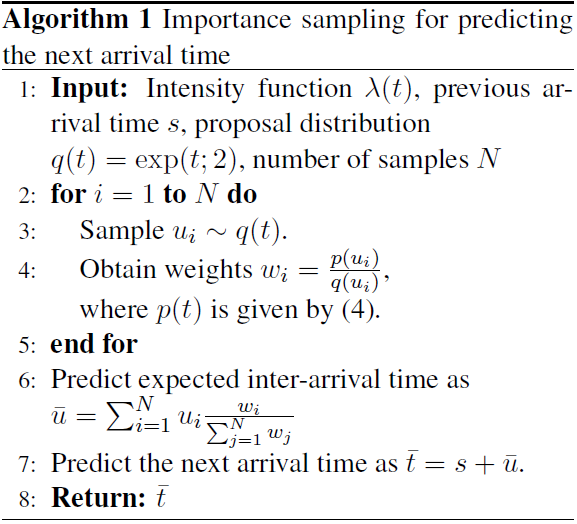
\includegraphics[width=\columnwidth]{importance sampling.PNG}
\end{flushleft}
\end{figure}
\end{column}
\begin{column}{0.5\textwidth}
\begin{enumerate}
    \item Sampling the inter-arrival time of occurrence of the next tweet using \eqref{eq:inter arrival time}. $p\brak t$ is given by \eqref{eq:inter arrival time}
    \item Proposal distribution is $Exp\brak{rate= 2}$\\ 
    $\therefore Mean=0.5$ 
    \item Assuming the previous tweet occurred at time $s$, the arrival time of next tweet is obtained using Algorithm 1.
    \item This algorithm is run sequentially until the end of the interval of interest is arrived.
\end{enumerate}
\end{column}
\end{columns}
\end{frame}

\begin{frame}{Incorporating Text}
\begin{enumerate}
    \item Kernel for text is a linear kernel:  $\vec{k_{text}\brak{x,x'}} = b + c \vec{x^T x'}$.
    \item The full kernel is: 
    \begin{align}
        \vec{k_{TXT}\brak{\brak{t,i},\brak{t',i'}}}= \vec{k_{time}\brak{t,t'}} + \vec{k_{text}\brak{x,x'}}
    \end{align}
\end{enumerate}

\textbf{Optimization:} All model parameters $\brak{a,l,b,c}$ are obtained using Maximum Likelihood Estimate(MLE) of the marginal likelihood over all rumour datasets.
\end{frame}

\begin{frame}{Experiments}
\begin{block}{Data pre-processing}
    \begin{enumerate}
        \item First 2 hours of each rumour lifespan is considered.
        \item Posts from first hour of target rumour is used for training.
        \item The arrival times of tweets in the second hour are predicted.
        \item They consider observations over equal sized time intervals of length 6 minutes in the rumour lifespan for learning the intensity function.
    \end{enumerate}
\end{block}
\begin{block}{Evaluation metrics}
        Two metrics based on root mean squared error (RMSE): aligned root mean squared error (ARMSE), penalized root mean squared error (PRMSE).
\end{block}
\begin{block}{Baselines}
    Homogeneous Poisson Process(HPP), Gaussian Process(GP) with linear kernel(GPLIN), Hawkes Process(HP).   
\end{block}
\end{frame}

\begin{frame}{Results}
\begin{figure}
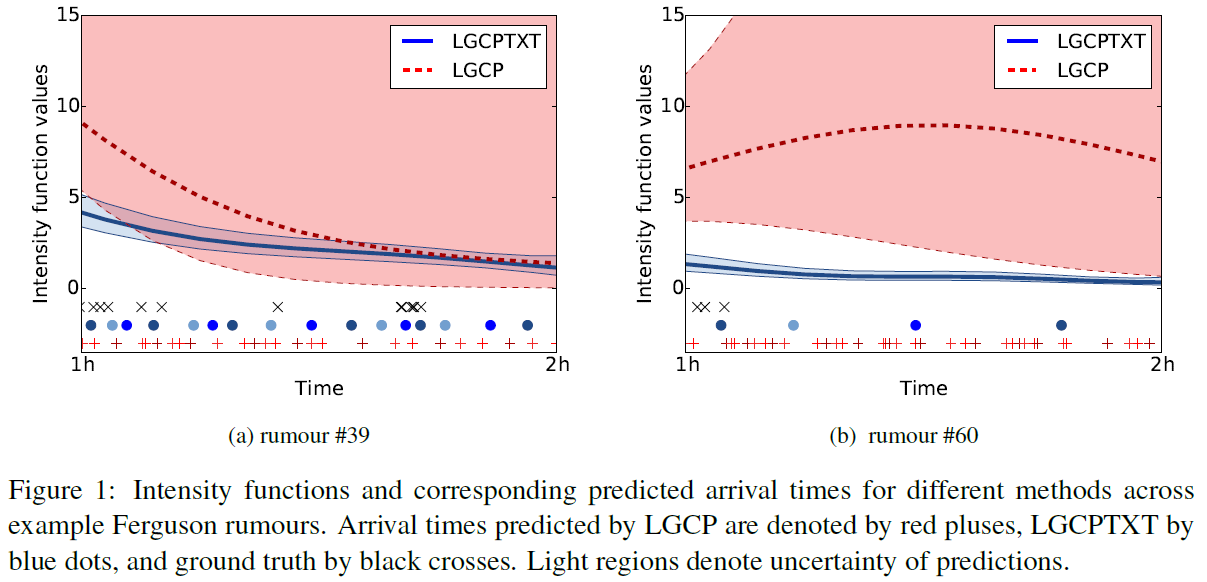
\includegraphics[width=\columnwidth]{predictions.PNG}
\label{results}
\end{figure}
\end{frame}

\begin{frame}{Contributions and Conclusion}
\begin{block}{This paper makes the following contributions:}
\begin{enumerate}
    \item Introduces \textbf{log-Gaussian Cox process} to predict tweet arrival times.
    \item Demonstrates how \textbf{incorporating text} improves results of inter-arrival time prediction.
    \item Evaluation on a set of rumours from Ferguson riots showed \textbf{efficacy of the proposed methods} comparing to baselines.
    \item Even though the central application is rumours, one could apply the proposed approaches to model the arrival times of tweets corresponding \textbf{to problems other than rumours}, e.g. disaster management, advertisement campaigns, discussions about politics
\end{enumerate}
\end{block}
\end{frame}

\end{document}
